\documentclass[11pt]{article}
\usepackage[utf8]{inputenc}
\usepackage[english, ngerman]{babel}
\usepackage{amsmath,amsthm,verbatim,amssymb,amsfonts,amscd}
\usepackage{enumerate}
\usepackage{listings}
\usepackage{courier}
% \usepackage{epstopdf}
\usepackage{graphicx}
\usepackage[margin=1in]{geometry}
\lstset{
  numbers=left,
  language=C,
  basicstyle=\footnotesize\ttfamily,
  breaklines=true,
  morekeywords={function, NIL}
}
\newcommand{\abs}[1]{\left| #1 \right| }
\setlength{\parindent}{0pt} 

\author{
  Felix Schrader, 3053850 \\ 
  Jens Duffert, 2843110 \\
  Eduard Sauter, 3053470
}
\title{Datenstrukturen und Algorithmen: Haus\"ubung 9}
\begin{document}
\maketitle
\subsection*{Aufgabe 2}
\begin{enumerate}[a)]
  \item $ $
    \begin{figure}[h!]
      \centering
      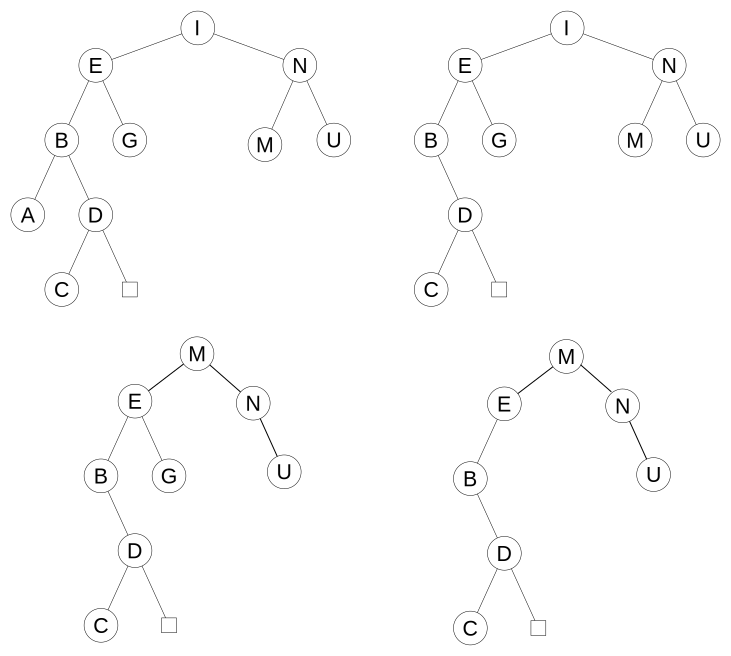
\includegraphics[width=0.8\textwidth]{avl_search_tree_delete}
      \caption{Löschen von A, I, G}
    \end{figure}
    
  \item $ $

    \begin{figure}[h!]
      \centering
      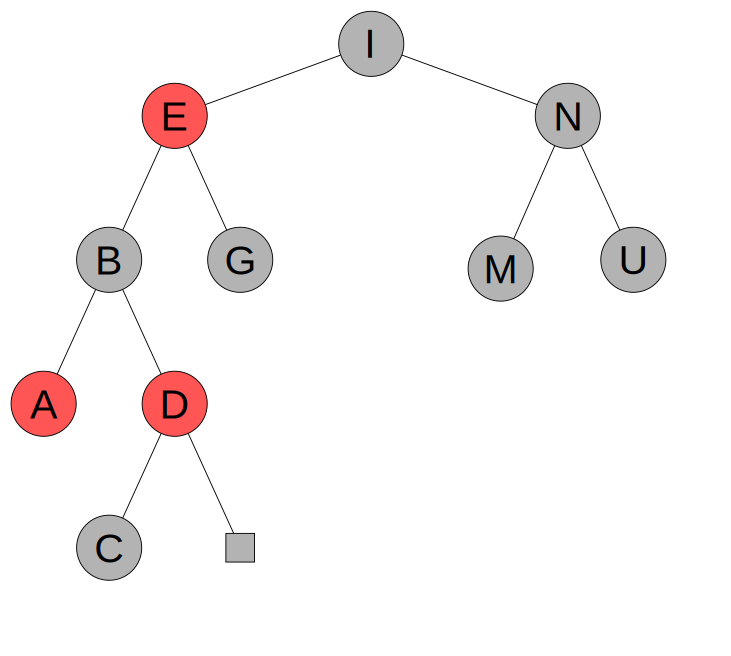
\includegraphics[width=0.4\textwidth]{avl_search_tree_red_black}
      \caption{Rot-Schwarz Version des Baumes}
    \end{figure}
    
  \item $ $

    \begin{figure}[h!]
      \centering
      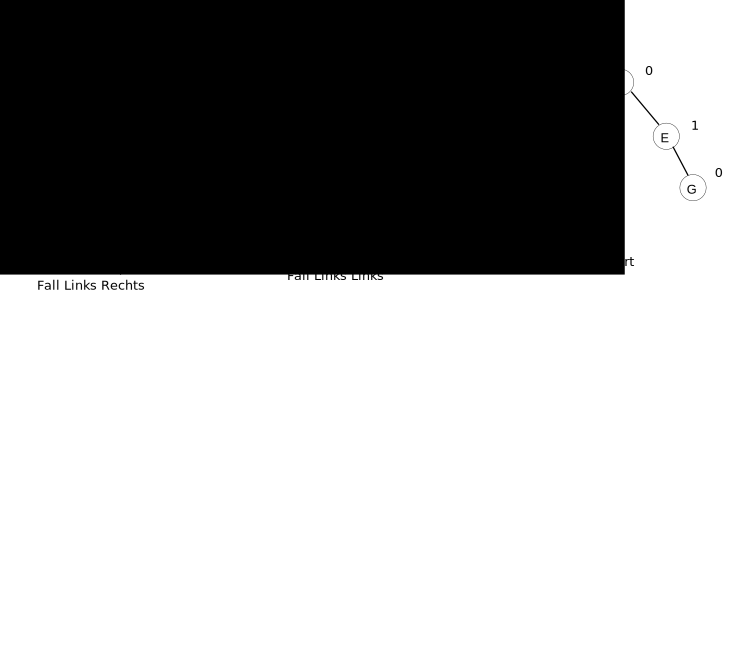
\includegraphics[width=0.8\textwidth]{avl_search_tree_rotate}
      \caption{AVL Rotationen}
    \end{figure}
    
\end{enumerate} 

\end{document}
